\documentclass[10pt]{exam}
\usepackage[phy]{template-for-exam}
\usepackage{tikz}
\usetikzlibrary{patterns}

\title{Marble Lab - MAKEUP IF ABSENT}
\author{Rohrbach}
\date{\today}

\begin{document}
\maketitle

\begin{questions}
  	
  \question
    In the lab, we rolled a marble down a ramp and let it hit the floor.  Assume that the initial velocity of the marble as it left the table was 2.4 m/s and that the table is 0.83 m tall.  Indicate your positive $x$- and $y$- direction on the diagram and use it to calculate where the marble should land.  
    
    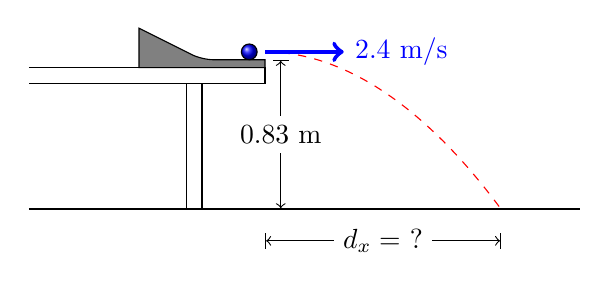
\begin{tikzpicture}
      \draw[thick] (0,0) -- (7,0);
      \draw (0,1.8)
        -- ++ (3,0)
        -- ++ (0,-.2)
        -- ++ (-3,0);
      \draw (2,0) rectangle (2.2,1.6);
      \draw[fill=gray] (3,1.9)
        -- ++(0,-.1)
        -- ++(-1.6,0) 
        -- ++(0,0.5)
        to[rounded corners] ++(.8,-.4)
        -- cycle;
      \draw[|<->|] (3.2,0) -- ++(0,1.9) 
        node[midway,fill=white] {0.83 m};
      \draw[shading=ball] (2.8,2) circle (0.1);
      \draw[dashed,red] (3,2) parabola (6,0);
      \draw[blue,ultra thick,->] (3,2) -- ++(1,0) 
        node[anchor=west] {2.4 m/s};
      \draw[|<->|] (3,-.4) -- ++(3,0) 
        node[midway,fill=white] {$d_x=$ ?};

    \end{tikzpicture}
  
  \question
    Which direction is the marble travelling right when it leaves the table?  Would you call this the $x$-direction or the $y$-direction?
    \vspace{3em}
  
  \question
    What are our knowns (what do we already know, or can easily measure)?

    \begin{center}
      \begin{tabular}{c|c}
        $x$-direction & $y$-direction \\
        \hline \\
        \\[5em]
      \end{tabular}
    \end{center}
  
  \question
    For what values do we need to solve?
    \vspace{3em}
  
  \question
    How can we solve for the $x$-displacement of the marble?  Try it:

  \pagebreak
  
  
  \uplevel{\section*{Conclusion}}
  
  \question
    What is the only variable that is the same in both the $x$- and the $y$- directions?  Why does it make sense that this variable is the same?
    \vs
  
  \question
    To find how far a projectile goes, you will usually solve this in two steps.  What are the two steps?
    \vs
\end{questions}





\end{document}